\documentclass{scrartcl}
\usepackage[mathletters]{ucs}
\usepackage[utf8x]{inputenc}
\usepackage{amssymb}
\usepackage{amsmath}
\usepackage[usenames]{color}
\usepackage{hyperref}
\usepackage{wasysym}
\usepackage{graphicx}
\usepackage[normalem]{ulem}
\usepackage{enumerate}

\usepackage{listings}

\lstset{ %
basicstyle=\footnotesize,       % the size of the fonts that are used for the code
showspaces=false,               % show spaces adding particular underscores
showstringspaces=false,         % underline spaces within strings
showtabs=false,                 % show tabs within strings adding particular underscores
frame=single,                   % adds a frame around the code
tabsize=2,                      % sets default tabsize to 2 spaces
breaklines=true,                % sets automatic line breaking
breakatwhitespace=false,        % sets if automatic breaks should only happen at whitespace
}


\title{2 camera position top}
\date{dinsdag 08 december 2020}
\author{}

\begin{document}

\maketitle

		\section{2 camera position top}

Created woensdag 11 november 2020



The same plates where used 04 -\textgreater{} 1until 5. 

Every pair of led is lighted separately to generate the photo's 



extra documents of the results in the folders images/dataset/.....



\subsection{Camera position to top}

The second test was conducted with the camera mounted a little more to the top of the inserts. This made the reflection from the worn area to the camera better. 

The first test results where also all black pictures caused by the same problem as on the first test of \href{./1_camera_position_side.tex}{camera position side}. On a second test this issue was resolved and the following pictures where the result. The issue was resolved by adding enormous amounts of delay for each command sent to the arduino. This made the process take very long (about 1 second per photo).



One picture was taken for every two leds of the strip with red light. for batch number 4 insert 3 with leds 5,6 and 7 turned on.



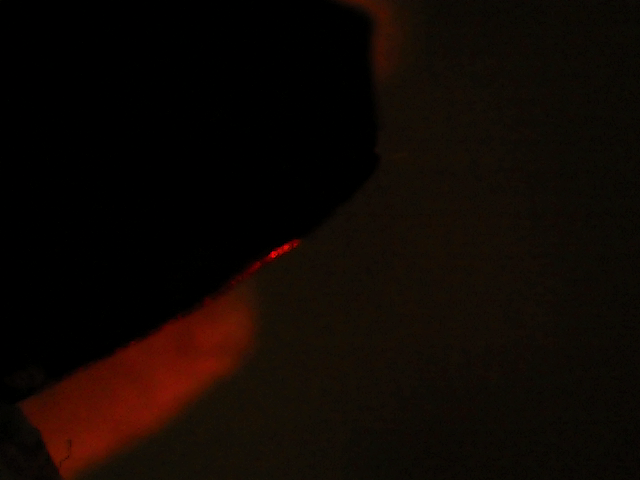
\includegraphics[width=3.125000in, keepaspectratio=true]{./2_camera_position_top/p3_l5.png}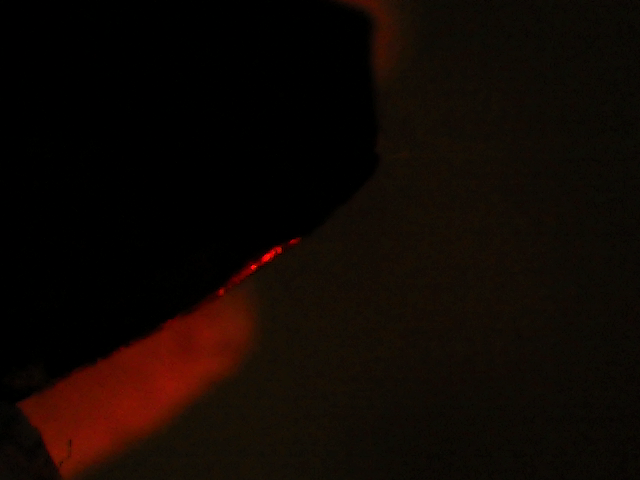
\includegraphics[width=3.125000in, keepaspectratio=true]{./2_camera_position_top/p3_l6.png}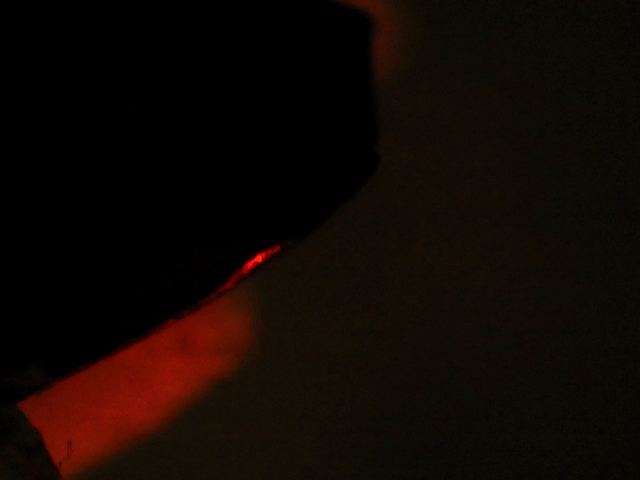
\includegraphics[width=3.125000in, keepaspectratio=true]{./2_camera_position_top/p3_l7.png}

On this data we can see the leds going up on the insert wear area. Which is what we tried to obtain. Now the leds are mapped to specific positions on the inserts and the amount of leds that need to be turned on for taking pictures can be reduced so no extra time is wasted. 





\end{document}
